% !TEX root = twibop2.tex
\chapter{Probability in Classical Physics}
\epigraph{Probability theory is used in physics, and its first application of fundamental importance for our understanding of the laws of nature can be found in the general statistical theory of heat founded by Boltzmann and	 Gibbs \ldots{} 
The most elegant and important advantage of this theory is the understanding of thermodynamical ``irreversibility'' as a picture of transition to more probable states.}  {W. Pauli}

\section{Thermodynamics and Its Puzzles }


All bodies consist of molecules in chaotic thermal motion. This fundamental point can be disregarded when considering the basic problems of \redem{thermodynamics}, the branch of physics which seeks to derive, from a few basic postulates, relationships between the properties of matter, especially those which are affected by changes in temperature, and a description of the conversion of energy from one form to another.

Thermodynamics is a branch of physics in which the energy transfers between macroscopic bodies and their environment are investigated from the most general positions (without using molecular concepts). Thermodynamic considerations are underlain by a description of the states of the bodies using thermodynamic \redem{variables or the thermodynamic functions of state} or state parameters, and the use of several basic principles called the \redem{laws of thermodynamics}. You already know about such thermodynamic variables as \redem{temperature} and \redem{pressure}.

\txthead{Thermodynamic equilibrium.} Let us perform a simple experiment. Take a vessel with hot water into a room and put a thermometer into the water. By recording the readings of the thermometer over time, we will see that the temperature of the water gradually decreases until finally equals the air temperature in the room, after which the temperature will remain constant. This means that the water in the vessel has reached a \redem{thermodynamic (heat) equilibrium} with the environment. If a system is in a thermodynamic equilibrium, its thermodynamic functions of state (temperature and pressure) remain constant until disturbed. Another feature of a thermodynamic equilibrium is that the temperature is constant at all points of the system.


If a system does not exchange energy with bodies around it, it is a \redem{closed system}. When we talk about a thermodynamic equilibrium of a closed system, we mean an equilibrium between its various parts, each of which can be regarded as a macroscopic body.

Suppose we heat a body unevenly and then put it in a vessel which does not conduct heat. It can be said that we first disturb the thermodynamic equilibrium in the body and then leave it. The temperature of the hotter regions will decrease, and that of cooler ones will increase, and finally the temperature will become the same throughout the body: they will reach a thermodynamic equilibrium with each other. \redem{An unperturbed macro-system will always reach a state of thermodynamic equilibrium and remain there} until some external action brings it out of this state. If this action stops, the system will again reach a thermodynamic equilibrium.


And here is the first puzzle of thermodynamics. Why does a system brought out of thermal equilibrium and left to itself return to an equilibrium state, while systems in a thermal equilibrium and left to themselves do not leave it? Why is it not necessary to spend energy to maintain thermal equilibrium, while energy is needed to maintain a system in a thermodynamic equilibrium? By the way, this is a far from futile question. The weather outside may be below freezing, e.g. \SI{-1}{\degreeCelsius}, while it's warm in the room, \SI{+25}{\degreeCelsius}. The walls of houses conduct heat fairly well, and therefore, there is a non-equilibrium ``room-outside'' system. To maintain this thermodynamic non-equilibrium state, it is necessary to spend energy continuously to heat.

\txthead{The first law of thermodynamics.} A system may exchange energy with its environment in many ways, or, as is said, along many channels. For simplicity's sake, let us limit ourselves to a consideration of two channels, namely, the transfer of energy by \redem{heat conduction} and the transfer of energy by \redem{performing work}. The \redem{first law of thermodynamics} is simply the law of the conservation of energy involving the possible energy transfer between a body and its environment via different channels, i.e.
\begin{equation}%
\Delta \, U = A + Q,
\label{eq-4.1}
% eq 4.1
\end{equation}
where $ \Delta \, U = U_{2} - U_{1}$ is the change in the internal energy of the body ($U_{1}$ and $U_{2}$ being the internal energies of the initial and final states of the body, respectively), $A$ is the work performed by external forces with respect to the body, and $Q$ is the amount of heat transferred to or from the body by conduction. Note that unlike internal energy, which is a \redem{function of state} of the body (it varies when the body transfers from one state to another), neither work nor heat are functions of state. It is equally absurd to say that a body in a state has so much heat or so much work. The heat $Q$ and work $A$ in formula \eqref{eq-4.1} are the changes in the body's energy carried out through different channels. Let us consider a simple macro-system, an \redem{ideal gas} ($m$ is the mass of the gas). The internal energy of an ideal gas is proportional to the absolute temperature $T$ of the gas and does not depend on the volume $V$ it occupies. Let us change the gas volume using a piston. By pushing a close-fitting piston down a cylinder and thus compressing the gas in the cylinder, we perform some work $A$. When the gas expands, it performs	work 	$A'$ to move the piston back: $A' = - A$. This work is related to the change in the gas volume. It is numerically equal to the area under the pressure-volume curve, which describes the process, from $V= V_{1}$ to $V= V_{2}$, where $V_{1}$ and $V_{2}$ are the initial and final volumes of the gas.

Let us consider, from the viewpoint of the first law of thermodynamics, two types of gas expansion, \redem{isothermal} and \redem{adiabatic}. The former process occurs at constant gas temperature while the latter occurs when there is no heat exchange between the gas and the environment. The change in the gas volume should be carried out very slowly (compared to the rate at which thermal equilibrium is reached within the gas), and so the gas can be regarded at any moment in time as being in thermodynamic equilibrium. In other words, we assume that the gas passes from one thermodynamic equilibrium state to another, as it were, via a succession of intermediate equilibrium states.

If the expansion is \redem{isothermal}, the gas's temperature remains constant, and therefore, $\Delta U = 0 \,\, (U_{1} = U_{2})$. Noting this, we obtain from \eqref{eq-4.1}:
\begin{equation}%
- A = Q \quad \textrm{or} \quad A' = Q.
\label{eq-4.2}
\end{equation}
The expanding gas performs as much work as it receives heat from the environment during its expansion.

When the expansion is \redem{adiabatic}, there is no heat exchange with the environment ($Q = 0$). Therefore,
\begin{equation}%
\Delta \, U = A \quad \qor \quad A' = - \Delta \, U.
\label{eq-4.3}
\end{equation}
The expanding gas performs work owing to a decrease in its internal energy, and the gas's temperature therefore falls.

\begin{marginfigure}[-3.5cm]%[!ht]
\centering
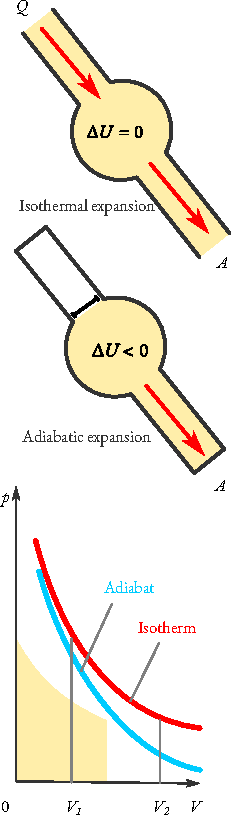
\includegraphics[width=0.8\textwidth]{figures/isotherm-adia.pdf}
\caption{Isothermal and adiabatic processes.\label{iso-adia}}
\end{marginfigure}


Both of these processes are conventionally shown in \figr{iso-adia}. The processes are also represented on $p-V$ diagrams (where $p$ is the gas pressure). The work $A'$ performed by the gas in an isothermal expansion from volume $V= V_{1}$ to $V= V_{2}$ equals numerically the yellow area under the plot of $p (V)$ in the figure:
\begin{equation}%
A' = \int\displaylimits_{V_{1}}^{V_{2}} p(V) \, \dd V.
\label{eq-4.4}
\end{equation}
Using an equation of state for an ideal gas (the Mendeleev-Clapeyron equation), we get
\begin{equation}%
p= \frac{mRT}{MV},
\label{eq-4.5}
\end{equation}
where $M$ is the molar mass of the gas and $R$ is the universal gas constant. Substituting \eqref{eq-4.5} into \eqref{eq-4.4} and given that the temperature of the gas is constant, we obtain
\begin{equation}%
A = \frac{mRT}{MV} \int\displaylimits_{V_{1}}^{V_{2}} \frac{1}{V} \,\, \dd V = \frac{mRT}{MV} \, \ln \frac{V_{2}}{V_{1}},
\label{eq-4.6}
% eq 4.6
\end{equation}
(the symbol $\ln$ designates a logarithm to base $e = 2.71828 \ldots{}$). 



\txthead{The Carnot cycle.} In 1824, a 28-year-old engineer called Sadi, Carnot published a book in Paris entitled \redem{Refl\'exions sur la puissance moteurice du feu et Ie machine propre \`a developper cette puissance} (Reflections on the Driving Force of Fire and Machines Capable of Developing This Force). Unfortunately, his ideas as presented in the book were only appreciated many years later, and long after he had died. Carnot was investigating the work obtained from heat engines. He showed that a heat machine not only needs a hot body, it also requires a second body with a lower temperature. The first body is conventionally called the heat source, and the second is called the heat sink. Besides the heat source and heat sink, there must be a working substance (a liquid, steam, or gas), which transmits the heat from the heat source to the heat sink and performs work in the process. Carnot considered a closed cycle consisting of two isotherms and two adiabats. Later this cycle was called the \redem{Carnot cycle}. It is shown in \figr{ideal-gas} for an ideal gas. 

\begin{marginfigure}%[!ht]
\centering
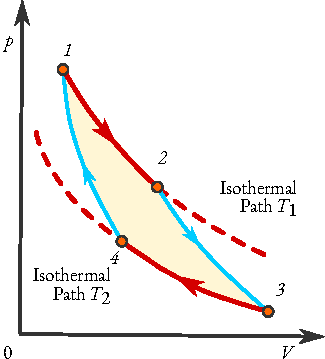
\includegraphics[width=\textwidth]{figures/carnot.pdf}
\caption{Carnot cycle for an ideal gas.\label{ideal-gas}}
\end{marginfigure}

Suppose $T_{1}$, is the temperature of the heat source and $T_{2}$ is that of the heat sink. Moving from point 1 to point 2 (the isotherm for $T_{1}$ ), the gas receives a heat $Q_{1}$ from the heat source and expands, thus spending energy to perform work $A$. From point 2 to point 3 (along an adiabat), the gas performs work $A$; and its temperature falls to $T_{2}$. From point 3 to point 4 (the isotherm for $T_{2}$) the gas gives a heat $Q_{2}$ to the heat sink, and this heat equals the work $A_{2}$ performed to compress the gas. From point 4 to point 1 (another adiabat), the work $A_{4}$ is expended to compress the gas, and this goes to increasing the internal energy of the gas, so its temperature rises to $T_{1}$. The result is that the working substance returns to its initial state 1. 

Suppose that a heat engine operates following the Carnot cycle. The gas receives a heat $Q_{1}$ from the beat source and gives a heat $Q_{2}$ to the heat sink. In compliance with \eqref{eq-4.2}, we can write $Q_{1} = A'$ and $|Q_{2}| = A_{2}$. Note here that $Q > 0$ when heat is given to the gas, and that $Q < 0$ when the heat is taken from the gas. It is clear from \hyperref[ideal-gas]{Figure \ref{ideal-gas}} that the area under isotherm 3-4 is smaller than that under isotherm 1-2, and therefore, $A_{2} < A_{1}'$. Consequently, $|Q_{2}| < Q_{1}$ i.e. the gas gives the heat sink less heat than it receives from the heat source. At the same time, the internal energy of the gas, when the cycle is completed, remains the same. Therefore, the difference $Q_{1} - |Q_{2}|$ equals the work performed by the heat engine during its cycle. Hence the
efficiency of the heat engine is 
\begin{equation}%
\eta = \frac{(Q_{1} - |Q_{2}|)}{Q_{1}}.
\label{eq-4.7}
\end{equation}
Carnot showed that
\begin{equation}%
\frac{Q_{1}}{T_{1}} = \frac{(|Q_{2}|)}{T_{2}}.
\label{eq-4.8}
\end{equation}
This allows us to rewrite \eqref{eq-4.7} in the form 
\begin{equation}%
\eta = \frac{(T_{2} - T_{1})}{T_{1}}.
\label{eq-4.9}
\end{equation}
The efficiency of a heat engine, as defined by \eqref{eq-4.7} and \eqref{eq-4.9}, is the best possible efficiency. The efficiency of real heat engines is always less because of unavoidable irreversible processes.

\txthead{Reversible and irreversible processes.} The notions of reversible and irreversible processes are essential for thermodynamics. A process is said to be \redem{reversible} if the system (the working substance) is in thermal equilibrium all the time, continuously passing from one equilibrium state to another. This process is completely controlled, while it lasts, by the changes in its parameters, for instance, the temperature or volume. If the parameters are changed in the reverse direction, the process will also go backwards. Reversible processes are also called \redem{equilibrium processes}.

Boyle's (Mariotte's) and Gay-Lussac's (Charles') laws define reversible processes in an ideal gas. The expressions \eqref{eq-4.7} and \eqref{eq-4.9} we have just obtained are related to a reversible Carnot cycle, which is also called the ideal Carnot cycle. Each part of the cycle and the whole cycle can be reversed if desired.

An \redem{irreversible} process is a process that cannot be controlled. It proceeds independently, or, in other words, spontaneously. The result is that we cannot reverse such a process. It was noted above that once a system is moved from its thermodynamic equilibrium, it tends spontaneously to another thermodynamic equilibrium state. Processes related to transition of a system from a non-equilibrium state to an equilibrium one are irreversible. They are also called \redem{non-equilibrium} processes.

Here are some examples of irreversible processes: conduction of heat from a hotter body to a cooler one, mixing of two or more gases in the same vessel, expansion of a gas in vacuum. All of these processes occur spontaneously, without any external control. Heat does not spontaneously transfer from a cooler body to a hotter one. The components of a gas mixture do not spontaneously separate. A gas cannot spontaneously compress. I wish to emphasize: \redem{every irreversible process is characterized by a definite direction}. It develops in a certain direction and does not develop in the opposite one. Which direction a process can develop along and which it cannot are problems related to the second law of thermodynamics.

\txthead{The second law of thermodynamics.} One of the first formulations of the \redem{second law of thermodynamics} was given by the English physicist William Thompson (Lord Kelvin):
\begin{quote}
``It is \redem{not} possible that, at the end of a cycle of changes, heat has been extracted from a reservoir and an equal amount of work has been produced without producing some other effects.''
\end{quote}
This means that it is impossible to design a machine to carry out work by reducing the internal energy of a medium, sea water, for instance. Kelvin called such a machine a \redem{perpetuum mobile of the second kind}. While some \redem{perpetua mobile} violate the law of the conservation of energy (\redem{perpetua mobile of the first kind}), those of the second kind do not contradict the first law of thermodynamics; they are instead forbidden by the second law.	

In 1850, the German physicist Rudolf Clausius formulated the second law of thermodynamics as follows: 
\begin{quote}
``The transfer of heat from a cooler body to a hotter one cannot proceed without compensation.'' 
\end{quote}
It is useful to demonstrate the equivalence of the formulations given by Kelvin and Clausius. If we could, despite Kelvin's formulation, ``extract'' heat from a medium and, using a cyclic process, turn it into work, then, using friction, transform this work into heat at a higher temperature, we would contradict Clausius's formulation because it would involve the conduction of heat from a cooler body to a hotter one within a closed cycle without any external force performing work.

On the other hand, suppose that, despite Clausius's formulation, we succeed in getting some quantity of heat $Q$ to conduct itself from a cooler body (at a temperature $T_{2}$) to a hotter one ($T_{1}$), and subsequently, allow this heat to go naturally from the hotter body to the cooler at the same time performing some work $A'$ while the rest of the heat $Q_{1} = Q - A'$ returns to the cooler body. This process is shown in \figr{perp}~\drkgry{(a)}. It is clear that this process corresponds to direct transformation of heat $Q - Q_{1}$ into work $A$ (\figr{perp}~\drkgry{(b)}), which evidently contradicts Kelvin's formulation.

\begin{marginfigure}[-2cm]%[!ht]
\centering
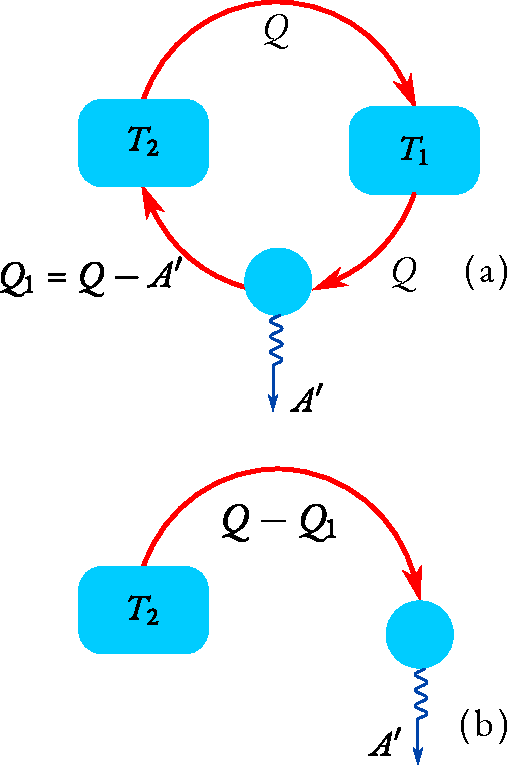
\includegraphics[width=\textwidth]{figures/perp.pdf}
\caption{Work done in transfer of heat from bodies at different temperatures.}
\label{perp}
\end{marginfigure}

\txthead{Entropy.} As he was studying Carnot's investigations, Clausius discovered that relationship \eqref{eq-4.8} is similar to a conservation law. The value of $Q_{1}/T_{1}$ ``taken'' by the working substance from the heat source equals the  $|Q_{2}|/T_{1}$ ``conducted'' to the heat sink. Clausius postulated a variable $S$, which like the internal energy is a state function of the body. If the working substance (an ideal gas in this case) receives heat 
$Q$ at temperature $T$, then $S$ is incremented by
\begin{equation}%
\Delta S= Q/T.
\label{eq-4.10}
\end{equation}
Clausius called $S$ \redem{entropy}. 

From point 1 to point 2 of the Carnot cycle (see \figr{ideal-gas}), a heat $Q_{1}$ is conducted from the, heat source to the working substance at a temperature $T_{1}$, and the entropy of the working substance increases by $\Delta S_{1} = Q_{1}/T_{1}$. From	 point 2 to point 3	and from point 4 to point 1, there is no conduction of heat, and therefore, the entropy of the working substance does not vary. From point 3 to point 4, a heat $Q_{2}$ is conducted from the working substance to the heat sink at temperature $T_{2}$, and	the	entropy of the	body is decreased by	$| \Delta S_{2}| = |Q_{2}| /T_{2} \,\, (\Delta S_{2} < 0)$. According to \eqref{eq-4.8} and \eqref{eq-4.10}), 
\begin{equation}%
\Delta S_{1} + \Delta S_{2} = 0.
\label{eq-4.11}
% eq 4.11
\end{equation}
Consequently, when an ideal (reversible) Carnot cycle comes to an end, the working substance's entropy returns to its initial value. 

Note that entropy can be defined as the state function of a body (system) whose value remains constant during an adiabatic process. Similarly, temperature can be regarded as the state function of a system whose value remains constant during an isothermal process. 

We shall later need to deal with a property of entropy called its additivity. This means that the entropy of a system is the sum of the entropies of the system's parts. Mass, volume, and internal energy are also additive. However, neither temperature nor pressure are additive.

\txthead{The second law of thermodynamics as the law of increasing entropy in irreversible processes within closed systems.} Using the notion of
entropy, we can formulate the second law of thermodynamics as follows:
\begin{mybox}{}
Any irreversible process in a closed system proceeds so that the system's entropy increases.
\end{mybox}
Consider the following irreversible process by way of an example. Suppose a closed system consists of two subsystems 1 and 2 which are at temperatures $T_{1}$ and $T_{2}$, respectively. Suppose that an infinitesimal amount of heat $\Delta Q$ is conducted from subsystem 1 to subsystem 2, so that the temperatures of the subsystems almost remain the same. The entropy of subsystem 1 reduces by $ \Delta Q/T_{1}$, $(S_{1} = - \Delta Q/T_{1})$ while the entropy of subsystem 2 increases by $\Delta S_{2} = \Delta Q/T_{2}$ The entropy of the whole system is the sum of its subsystems' entropies, and therefore, the change in the system's entropy will be
\begin{equation}%
\Delta S =  \Delta S_{1} + \Delta S_{2} = \Delta Q \left( \frac{1}{T_{2}} - \frac{1}{T_{1}} \right).
\label{eq-4.12}
\end{equation}
Heat conduction from subsystem 1 to subsystem 2 is irreversible if $T_{1} > T_{2}$. Using this inequality, we can conclude from \eqref{eq-4.12} that $\Delta S > 0$. Thus, we see that the process of heat conduction from a heated body to a cooler one is accompanied by an increase in the entropy of the system consisting of the two.

A gain in entropy during irreversible processes is only a necessary law for closed systems. If a system is open, a reduction in its entropy is possible. Thus, if some external body does work with respect to the system, heat can be transferred from a heat sink to a heat source. It is essential that if the system includes a heat source, a heat sink, a working substance, and all the bodies that perform work (i.e. if we consider a closed system again), then. the total entropy of this system will increase.

I shall now formulate the basic conclusions concerning the change in the system's entropy.

\redem{The first conclusion.} If a system is closed, its entropy does not decrease over time:
\begin{equation}%
\Delta S \geqslant 0.
\label{eq-4.13}
\end{equation}
The system's entropy does not vary if the processes within it are reversible. If the processes are irreversible, the system's entropy increases. The gain in entropy can be regarded as a measure of the irreversibility of the processes occurring in it.

\redem{The second conclusion.} Generally, nothing can be said about the change in entropy in an open system. It can either remain constant or increase or even decrease.

\txthead{The puzzles of thermodynamics.} These puzzles focus on the second law of thermodynamics. Since it gives a definite direction to the processes in nature, it introduces a fundamental irreversibility. How can this irreversibility be explained by physics? Why can heat be transferred from a hotter body to a cooler one while it cannot be spontaneously conducted in the opposite direction? Why does any gas expand in vacuum but does not compress spontaneously? Why, when in the same vessel, do two or more gases mix, but not spontaneously separate? A hammer strikes an anvil. The temperature of the anvil rises a bit. But however strongly we might heat the anvil with the hammer resting on it, the reverse will not happen: the hammer will not jump off the anvil. Why? Very many similar ``whys'' can be asked. Thermodynamics does not answer these questions in principle. The answer must be sought in the kinetic theory of matter. We should now look into the picture of chaotically moving molecules.

\section{Molecules in a Gas and Probability }

\txthead{A dialogue with the author.} Imagine that we are talking with a physicist of the 1860s. We do not need a ``time machine''. We shall just believe that my partner adheres to the views typical of physicists in the mid-$19^{\text{th}}$ century, the same physicists, many of whom later, in the 1870s, could not understand or accept the ideas of the Austrian physicist Ludwig Boltzmann (1844-1906). Anyway, let us imagine that it is 1861. 

\begin{dialogue}

\athr ``Let us consider a gas to be an ensemble of very many
chaotically moving molecules.''

\prtnr ``Good. I'm aware of the recent investigations of James
Clerk Maxwell, who calculated the velocity distribution of molecules
in a gas.'' 

\athr ``I would like to discuss some thing more fundamental than
the distribution established by Maxwell. The point is that there is a qualitative difference between considering thermodynamic equilibria and considering the motion of molecules. In the first we have \redem{dynamic} laws with strictly determined dependences, and in the second we have the \redem{probabilistic} laws that govern processes in large ensembles of molecules.''

\prtnr	``But the movements of molecules are governed by Newton's laws of classical mechanics rather than by probabilistic laws. Suppose we assign coordinates and velocities to all the molecules in a gas at a certain moment. Suppose that we can follow all the collisions of the molecules with each other and with the walls of the vessel. It is clear that in this case we will be able to predict where a molecule will be at some other moment and what velocity it will have.''


\athr ``Why aren't you bothered by the fact that you're very much like the superbeing of which Laplace wrote?''

\prtnr ``I have a concrete problem in mechanics. True, the number of bodies is extremely great.''

\athr ``There are about \num{d19} molecules in a cubic centimetre of gas under normal conditions. You have a problem in which some \num{d20} bodies have to be accounted for.''

\prtnr ``Naturally, it would be exceptionally difficult. But the difficulty is purely technical and not fundamental. So long as our calculational abilities are limited, we shall have to resort to probabilities, the probability of a molecule arriving in a volume, its probability of having a velocity in a certain range, etc.''


\athr ``Thus, you believe that the use of probabilities is only related to our practical inability to perform a very cumbersome calculation, but that in principle an ensemble of molecules behaves according to Newton's laws as applied to individual molecules.''

\prtnr ``Precisely. This is why I do not see the qualitative difference you mentioned.''

\athr ``I have at least three hefty arguments to support my position that the probabilistic description of large ensembles of molecules is necessary in principle, that chance is present in the very nature of these ensembles rather than simply being related, as you seem to believe, with our inadequate knowledge and inability to perform cumbersome calculations.''

\prtnr ``I'd like to know of these arguments.''

\athr ``I'll start with the first. Suppose there is, as you postulate,
a rigid system of strictly determined links (as given by Newton's laws) between the molecules in a gas. Now imagine that some of these molecules suddenly escape from this system (e.g. they escape from the vessel through a slit). Clearly the disappearance of these molecules will bring about the disappearance of all that is predetermined by their presence, I mean their later collisions with other molecules, which, in its turn, will change the behaviour of the other molecules. All this will affect the whole system of rigid relationships and, as a consequence, the behaviour of the ensemble as a whole. However, we know that from the viewpoint of gas as a whole you can suddenly withdraw a large number of molecules without any noticeable effect (for instance, \num{d12} molecules or more). The properties of the gas and its behaviour do not change in the least. Does this not indicate that the dynamic laws governing the behaviour of individual molecules do not actually interfere with the behaviour of the gas as a whole?"

\prtnr ``Still, it is hard to believe that molecules obey some laws while the ensemble of the same molecules obeys quite different laws.''




\athr ``But this is exactly so. And my second argument will emphasize this fundamental point. I'll give you some simple examples. A stone is thrown from point $A$ at some angle to the horizontal (\figr{reflect}~\drkgry{(a)}). Imagine that we can change the direction of the stone's velocity to the opposite at point $B$ of its trajectory. It is clear that the stone should return to point $A$ and have the same velocity (in absolute value) it had when it was thrown. The flying stone, as it were, `remembers' its history.''

\prtnr ``This is natural because each state of the thrown stone is
determined by its preceding one and, in its turn, determines the subsequent one.''
\begin{marginfigure}%[!ht]
\centering
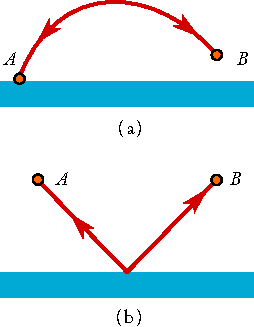
\includegraphics[width=\textwidth]{figures/reflect.pdf}
\caption{Bounce of a stone and an elastic ball.\label{reflect}}
\end{marginfigure}

\athr ``Another example: a ball hits a wall elastically and bounces
off (\figr{reflect}~\drkgry{(b)}). If you change the direction of the ball's velocity to the opposite one at point $B$, the situation will recur in the reverse order: the ball will hit the wall and return to point $A$.

``I cited these examples in order to illustrate an essential idea: the movements determined by the laws of classical mechanics have a kind of ``memory'' of the past. This is why these movements can be reversed.''

``Another thing is the behaviour of gas. Imagine the following situation. There is a beam of molecules whose velocities are parallel. After entering a vessel, the molecules collide many times with each other and the walls. The result is that the molecules reach a state of thermodynamic equilibrium, and they lose all `memory' of their past. It can be said that any gas in a state of thermal equilibrium, as it were, `forgets' its prehistory and does not `remember' how it arrived at the equilibrium state. Therefore, it is absurd to think of reversing the situation: the molecules could not recollect into a beam and depart from, the vessel in one definite direction. Many examples of such forgetfulness can be cited.''

``Suppose there is some gas on one side of a partition in a vessel and another gas is on the other side. If you take away the partition, the molecules of both gases will mix. Evidently, we should not expect this picture to reverse: the molecules will not move back into their own halves of the vessel. We might say that the mixture of two gases does not remember its prehistory.''

\prtnr ``Do you want to say that the equilibrium state of a gas is not predetermined by the preceding states of the gas?''

\athr ``When we use the word predetermined, we mean strictly unambiguous predetermination. There is no such predetermination here. A gas may arrive in an equilibrium state from different initial states. No information may be obtained about the initial states by studying the gas in thermal equilibrium. This means that the gas forgets its prehistory.''

\prtnr ``Yes, this is true.''

\athr ``And when does this loss of memory occur? It occurs when \redem{chance} comes into play. You throw a die, and, say, a four turns face up. You throw again and a two appears. The appearance of the two is not related to the appearance of the four before it. You throw the die many times and obtain a set of digits. This set possesses stability (for instance, the four occurs approximately in one-sixth of all trials). This stability does not have any prehistory, it is not related to the occurrence of any other digit in the previous trials.''

``The same happens in a gas. The loss of prehistory indicates that we must deal with \redem{statistical} laws, laws in which chance plays a fundamental role.''

\prtnr ``It seemed to me before that everything was clear. Newton developed his mechanics. Then the temperature and pressure of gas appeared. Using the notion of molecules, we reduced these physical variables to mechanical ones by relating temperature to the energy of molecules and the pressure of the gas to the impulses transferred to the wall by the molecules striking it. Therefore, the laws of mechanics were and continue to be fundamental laws. Are you suggesting we put probabilistic laws on the same level as the laws of mechanics?''

\athr ``I believe that you are aware of the fact that some thermodynamic variables do not have analogues in classical mechanics. And here is my third argument. Entropy does not have a mechanical analogue. The very existence of a variable such as entropy is sufficient to disprove the thesis of the total fundamentality of the laws of classical mechanics.''

\prtnr	``I would not like to discuss entropy at all \ldots{}'' 


\end{dialogue}

Let us finish with this dialogue because it has become a bit too long. We agreed that it referred to 1861. Therefore, I could not use arguments that were unknown at the time. But here I can cite two more arguments in favour of my position. Firstly, note that entropy is explicitly expressed in terms of probability, and that namely this makes it possible to explain every puzzle of thermodynamics. We shall discuss this in detail in the next sections. Secondly, it follows from quantum physics that the assumption (made by my partner) that he can assign coordinates and velocities to all the molecules simultaneously proves to be inconsistent. This cannot be done due to fundamental considerations, which we shall talk about in detail in Chapter 5. 

And now let us discuss molecules moving in a gas.

\txthead{Movements of gas molecules in thermodynamic equilibrium.} Suppose a gas of mass $m$ is in thermal equilibrium. The gas occupies volume $V$ and has temperature $T$ and pressure $p$.

Each gas molecule moves with a velocity which is constant in magnitude and direction until the molecule collides with either another molecule or the wall. On the whole, the picture of molecular movements is chaotic: the molecules move in different directions with different velocities, there are chaotic collisions leading to changes in the direction of movement and the absolute value of the velocities of molecules. Let us take an imaginary ``photograph'' of the molecules' positions at a single moment in time. It might look like the one in (\figr{mol-photo}), where for simplicity's sake only two rather than three dimensions are considered (the ``photograph'' is flat). It is clear that the points (molecules) fill the volume of the vessel uniformly (the vessel in the figure is the square). Suppose $N$ is the total number of molecules in the vessel; $N=N_{A}m /M$, where $N_{A}$ is Avogadro's number. At any site within the vessel and at any moment in time, the number of molecules per unit volume is the same (on average), $N/V$. Molecules may be found with equal probability at any point within the vessel.
\begin{marginfigure}%[!ht]
\centering
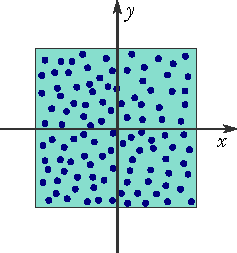
\includegraphics[width=0.95\textwidth]{figures/mol-photo.pdf}
\caption{A snapshot of the molecules in motion.\label{mol-photo}}
% fig 4.5
\end{marginfigure}

Let us use $G (x, y, z) \, \Delta dx \, \Delta dy\, \Delta dz$ to denote the probability of finding a molecule within a volume $ \Delta V = \Delta x \, \Delta y \, \Delta z$ in the vicinity of a point with coordinates $(x, y, z)$. To be more accurate, this is the probability that the $x$-coordinate of the molecule will take a value from $x$ to $x + \Delta x$, its $y$-coordinate from $y$ to $y + \Delta y$, and its $z$-coordinate from $z$ to $z + \Delta z$. At small $ \Delta x, \, \Delta y$, and $ \Delta z$, the function $G(x, y, z)$ will be the density of the probability of finding a molecule at point $(x, y, z)$. The probability density in this case does not depend on the coordinates, hence $G = \text{const}$. Since the probability of finding a molecule somewhere within the vessel is unity, we have
\begin{equation*}%
\int\limits_{V} G \, \dd V =1,  \qor  G \int\limits_{V}  \dd V = GV = 1.
\end{equation*}
Consequently, $G = 1/V$. 

Wherever a unit volume is taken within the vessel, the probability of finding a molecule within the unit volume is $1/V$, i.e. the ratio of the unit volume to the volume of the vessel. Generalizing this conclusion, we can state that the probability of finding a molecule within volume $V_{0}$ is $V_{0}/V$.

\begin{marginfigure}%[!ht]
\centering
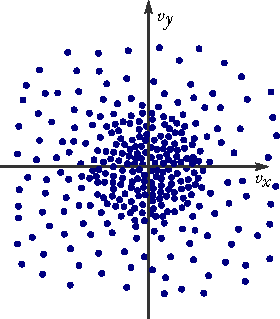
\includegraphics[width=\textwidth]{figures/mol-dist.pdf}
\caption{A snapshot of molecular velocity distribution.}
\label{mol-dist}
% fig 4.6
\end{marginfigure}

Now let us discuss the velocities of the gas molecules. It is clear from the start that the velocities cannot all be equally probable: there should be few molecules with very high and very small velocities. When considering the velocities of molecules, it is convenient to use the concept of a \redem{velocity space}, i.e. the molecular velocities are projected onto the coordinate axes $v_{x}, v_{y}, v_{z}$. For simplicity's sake, \figr{mol-dist} shows only two axes: the $v_{x}$-axis and the $v_{y}$-axis (a two-dimensional velocity space). The figure shows a molecular velocity distribution in a gas for some moment in time. Each point in the figure relates to a molecule. The abscissa of the point is the $x$-projection of the molecule's velocity and the ordinate is its $y$-projection.

It is interesting to compare \figr{mol-photo} and \figr{mol-dist}. The points in \figr{mol-photo} are within a certain area and the distribution is uniform. The scatter of points in \figr{mol-dist} is unlimited in principle. These points clearly focus around the origin. This means that although the projection of a molecule velocity may be as large as you wish, the projections of the velocities in the neighbourhood of zero are the most probable. The scattering in \figr{mol-dist} is rotationally symmetric for any angle about the origin. This means that all directions of movement are equally probable: a molecule may be found moving in any direction with equal probability.

In order to have a correct picture of the molecular movements in a gas, we should use both figures. It is still better, instead of each figure, to consider a sequence of snapshots taken at regular intervals in time.

We should then see that the points in \figr{mol-photo}  move in different directions: the trajectories change during collisions. The points in \figr{mol-dist} do not move; however, some suddenly disappear and some appear. Each time a pair of points disappears another pair of new points appears: this is the result of collision between two molecules.

\txthead{Maxwell's distribution law.} Suppose $F  (v_{x}) \Delta v_{x}$ is the probability that a certain molecule (at a certain moment in time) has an $x$-velocity component	from	 $v_{x}$	to	$v_{x} + \Delta v_{x}$	the	other two	velocity components taking any arbitrary value. At small $\Delta v_{x}$ the function $F  (v_{x})$ is the density of the probability of finding a molecule with velocity component $v_{x}$.

The English physicist James Clerk Maxwell (1831 -1879) showed that
the	probability	density	 $F  (v_{x})$ corresponds	to \redem{Gauss's law}:
\begin{equation}%
F (v_{x}) = A \, \exp (- \alpha \, v_{x}^{2}),
\label{eq-4.14}
\end{equation}
where $\alpha$ is a parameter ($\alpha > 0$) and the constant $A$ is determined from
\begin{equation}%
\int\limits_{- \infty}^{\infty} F (v_{x}) \dd v_{x} = 1,
\label{eq-4.15}
\end{equation}
which is a reflection of the fact that the probability of a molecule having
an $x$-component in its velocity is unity. Substituting \eqref{eq-4.14} into \eqref{eq-4.15}, we obtain
\begin{equation*}%
A \, \int\limits_{- \infty}^{\infty} \exp (- \alpha \, v_{x}^{2}) \dd v_{x} = 1.
\label{gauss-law-param}
\end{equation*}
The integral in this expression is known in mathematics as Poisson's integral and, evaluates to $\sqrt{\pi / \alpha}$. Consequently, $ A = \sqrt{\pi / \alpha}$. Thus, we can rewrite \eqref{eq-4.14} as 
\begin{equation}%
F (v_{x})  = \sqrt{\pi / \alpha} \, \exp (- \alpha \, v_{x}^{2}).
\label{eq-4.16}
\end{equation}
Similar functions can be derived for the probability densities for the $y$- and $z$-components of a molecule's velocity. The function $F(v_{x} )$ is plotted in \figr{gauss-dist}. Suppose $f \,(v_{x}, v_{y}, v_{z})$ is the density of the probability of finding a molecule with velocity components $v_{x}, v_{y}$, and $v_{z}$. Using the theorem of probability multiplication, we can write:
\begin{equation*}%
f \, (v_{x}, v_{y}, v_{z}) \, \Delta v_{x}\, \Delta  v_{y} \, \Delta v_{z} = [F(v_{x} \Delta \, v_{x})] [F(v_{y} \Delta \, v_{y})][F(v_{z} \Delta \, v_{z})].
\end{equation*}
Whence
\begin{equation}
f \, (v_{x}, v_{y}, v_{z}) = \left(\frac{\alpha}{\pi} \right) ^{3/2} \, \exp (- \alpha (v_{x}^{2}+ v_{y}^{2} + v_{z}^{2})) = \left(\frac{\alpha}{\pi} \right) ^{3/2} \, \exp(- \alpha v^{2}).
\label{eq-4.17}
\end{equation}

\begin{figure}[!ht]
\centering
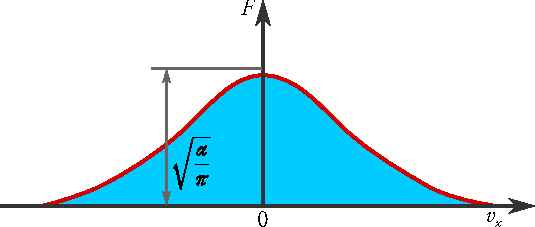
\includegraphics[width=0.75\textwidth]{figures/maxwl-dist1.pdf}
\sidecaption{The Gauss velocity distribution.\label{gauss-dist}}
\end{figure}



We see that the probability density depends on the squares of the velocity components, viz. $v_{x}^{2}+ v_{y}^{2} + v_{z}^{2}= v^{2}$. This we might have expected because, as it was already noted, each velocity direction is equally probable, and so the probability density may only depend on the absolute value of a molecule's velocity.

Thus, the probability of finding a molecule with velocity components taking the values $v_{x} - v_{x} + \, \Delta v_{x}, \,\, v_{y} - v_{y} + \, \Delta v_{y}, \,\,v_{z} - v_{z} + \, \Delta v_{z}, \,\,$ is:
\begin{equation}%
\Delta w_{v}  = \left(\frac{\alpha}{\pi} \right) ^{3/2} \, \exp (- \alpha v^{2})  \Delta v_{x} \Delta v_{y} \Delta v_{z},
\label{eq-4.18}
\end{equation}
where $v^{2} = v_{x}^{2}+ v_{y}^{2} + v_{z}^{2}$.

	
\begin{figure}[!ht]
\centering
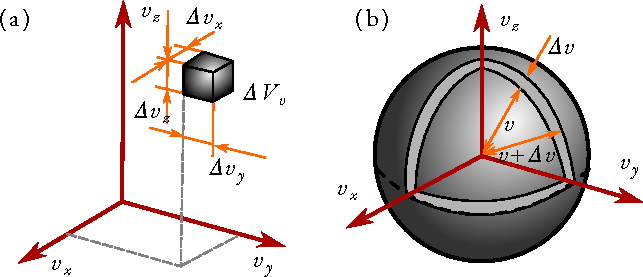
\includegraphics[width=0.9\textwidth]{figures/velspace.pdf}
\sidecaption{The velocity space.\label{vel-space}}
% fig 4.8
\end{figure}
Let us take one more step: since each velocity direction is equally probable, let us look at the probability of finding a molecule with an absolute	velocity from $v$ to $v + \Delta v$,	irrespective of	its direction. If	we consider a velocity space (\figr{vel-space}), then $\Delta w_{v}$ (see \eqref{eq-4.18}) is the probability of finding a molecule in the ``volume'' $\Delta v$, shown in (\figr{vel-space}~\drkgry{(a)}) (the word ``volume'' is enclosed in quotation marks to remind us that we are dealing with a velocity space rather than with a normal space). Now we want to consider the probability of finding a molecule within the spherical layer shown in \figr{vel-space}~\drkgry{(b)} and confined between spheres with radii $v$ and $v + \Delta v$. The ``volume'' of this layer is the surface area of a sphere of radius $v$ multiplied by the thickness of the layer $\Delta v$, i.e. $4 \pi v^{2} \Delta v$. Therefore, the probability we want has the form:
\begin{equation}%
\Delta w_{v}  = \left(\frac{\alpha}{\pi} \right) ^{3/2} \exp (- \alpha v^{2})  4 \pi v^{2} \Delta v.
\label{eq-4.19}
\end{equation}
This formula expresses the distribution of molecules in an ideal gas by the absolute value of their velocities, i.e. the \redem{Maxwellian distribution}. The probability density $g (v) = \Delta w_{v} / \Delta v$ is shown in \figr{mxwl-space}. It vanishes both when $v$ tends to zero and when it tends to infinity. The ``volume'' of the spherical layer shown in \figr{vel-space}~\drkgry{(b)} vanishes when $v$ tends to zero and the factor $\exp(- \alpha v^{2})$ in the distribution law vanishes when $v$ tends to infinity.
\begin{figure}[!ht]
\centering
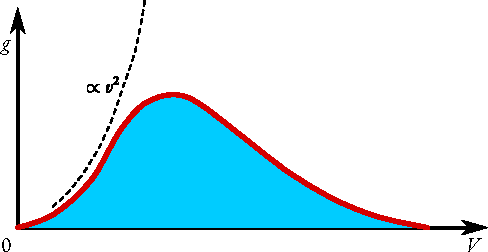
\includegraphics[width=0.8\textwidth]{figures/dist2.pdf}
\sidecaption{The Maxwellian velocity distribution.\label{mxwl-space}}
% fig 4.9
\end{figure}

\txthead{Chance and necessity in the pattern of moving molecules.} Suppose we could record the position and velocity of every molecule in a volume of gas at some moment in time. Imagine now that we divide the volume into numerous identical cells, and look at our instantaneous ``photograph'' from cell to cell. It will turn out that the number of molecules varies from cell to cell in a random fashion. Let us only pay attention to those molecules whose velocities are within the range from $v$ to $v + \Delta v$. The number of such molecules varies randomly from cell to cell. Let us divide the solid angle for all space at a point, i.e. $4 \pi$ steradians, into many identical elementary solid angles. The number of molecules whose velocities lie within an elementary solid angle varies randomly from one such an angle to another.

We could look at the situation in another way, that is, we could focus our attention on some cell or an elementary solid angle and take snapshots at different moments in time. The number of molecules (in a cell or a solid angle) at different times will also randomly change.

To emphasize the \redem{randomness} in the picture of moving molecules, the term ``chaotic'' is applied: chaotic collisions between molecules, chaotically directed molecule velocities, or generally, the chaotic thermal
movement of molecules. However, there is some \redem{order} in this ``chaos'' or, in other words, \redem{necessity} or what we have repeatedly called \redem{statistical stability}.

The statistical stability shows itself in the existence of definite probabilities: the probability of a molecule being in a volume $\Delta V$ (the probability is $\Delta V/ V$), the probability of a molecule moving within a solid angle $\Delta \Omega$ (the probability is $\Delta \Omega/4\pi$), and the probability of a molecule having an absolute value of velocity from $v$ to $v + \Delta v$ (the probability is defined by \eqref{eq-4.19}).

The number of molecules per unit volume each possessing an absolute value of velocity from $v$ to $v + \Delta v$ is, to a great degree of accuracy,
\begin{equation}%
\Delta n = \frac{N}{V} \, \Delta w_{v}  =  4 \pi \, \frac{N}{V}  \left(\frac{\alpha}{\pi} \right) ^{3/2} \, \exp (- \alpha v^{2}) \, 4 \pi v^{2} \Delta v.
\label{eq-4.20}
% eq 4.20
\end{equation}
Collisions between molecules push some molecules out of this range of velocity values; however, other collisions bring new molecules into it. So order is maintained: the number of molecules in a given interval of velocity values remains practically constant and is defined by \eqref{eq-4.20}. Let me emphasize that chance and necessity, as always, are dialectically united here. Collisions among a great number of molecules give the picture of the moving molecules its randomness. But at the same time the collisions maintain the thermodynamic equilibrium in the gas, which is characterized by definite probabilities, and in turn reveals statistical stability.

\section{Pressure and Temperature of an Ideal Gas}

\txthead{Pressure as the result of molecular bombardment.} The walls of a vessel containing a gas are continuously struck by gas molecules. This molecular bombardment results in the pressure exerted by a gas on a wall. Let us take an $x$-axis at right angles to the wall. It is clear from \figr{collisions}~\drkgry{(a)} that the $x$-component of a molecule's momentum in an elastic collision with the wall changes by $2m_{0}v_{x}$ where $m_{0}$ is the mass of the molecule. This means that when it strikes the wall, the molecule gives it an impulse of $2m_{0}v_{x}$. Let us first look at those gas molecules whose $x$-components of velocity lie between $v_{x}$ and $v_{x} + \Delta v_{x}$ (note that $v_{x} > 0$, otherwise the molecule will be moving away from the wall rather than towards it); the other components of the molecule's velocity are not important. The number of collisions between the molecules in question and an area $s$ of the wall per unit time equals the number of molecules in a volume equal to $s v_{x}$ \figr{collisions}~\drkgry{(b)}. (The reader should not be confused by the fact that the product $s v_{x}$ does not have the dimensions of volume. In reality, we deal herewith the product $s(\si{\centi\meter\squared}) \times v_{x} (\si{\centi\meter\per\second}) \times 1 (\si{\second})$.) Regarding \eqref{eq-4.16}), this number of collisions is
\begin{equation*}%
\Delta R = \frac{N}{V} \, s\, v_{x} F(v_{x}) \, \Delta v_{x} =  \frac{N}{V} \, s\, v_{x} \sqrt{\frac{\alpha}{ \pi}} \, \exp (- \alpha v_{x}^{2}) \, \Delta v_{x}.
\end{equation*}

\begin{figure}[!ht]
\centering
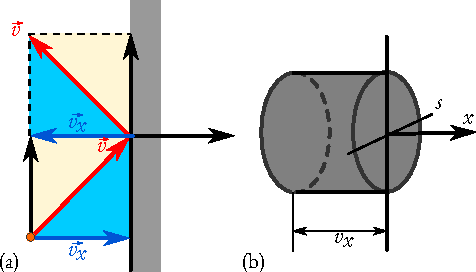
\includegraphics[width=0.8\textwidth]{figures/collisions.pdf}
\sidecaption{The collisions of molecules with walls of the container.\label{collisions}}
% fig 4.10
\end{figure}

The wall receives an impulse of  $2m_{0}v_{x}$ at each collision. The force acting on an area $s$ of the wall per unit time is the impulse transferred to the area. Dividing the force by the area $s$, we can find the pressure exerted by the gas on the wall caused by the molecules whose $x$-velocity components take values from $v_{x}$ to $v_{x} + \Delta v_{x}$:
\begin{equation}%
\Delta p = 2m_{0}v_{x} \Delta R  \frac{1}{s} =  2m_{0} \frac{N}{V} \, \sqrt{\frac{\alpha}{ \pi}} \exp (- \alpha v_{x}^{2}) \, v_{x}^{2} \, \Delta v_{x}.
\label{eq-4.21}
% eq 4.21
\end{equation}
The only thing left is to sum up, or, more accurately, to integrate \eqref
{eq-4.21} over all non-negative values of velocity $v_{x}$:
\begin{equation}%
p = 2m_{0} \frac{N}{V} \, \sqrt{\frac{\alpha}{ \pi}}  \int\limits_{- \infty}^{\infty} \exp (- \alpha v_{x}^{2}) \, v_{x}^{2} \, \dd v_{x}.
\label{eq-4.22}
% eq 4.22
\end{equation}
The following is a standard identity:
\begin{equation*}%
\int\limits_{0}^{\infty} \exp (- \alpha v_{x}^{2}) \, v_{x}^{2} \, d v_{x} = \frac{1}{4} \sqrt{\frac{ \pi}{\alpha^{3}}}.
\end{equation*}
Therefore, 
\begin{equation}%
p = m_{0}N /2 \alpha V.
\label{eq-4.23}
\end{equation}

\txthead{Maxwellian distribution finally becomes clear.} We have long tried the reader's patience with the mysterious parameter $\alpha$. It is clear from \eqref{eq-4.23} that $\alpha = m_{0}N /2pV$. Since the gas is in a thermal equilibrium, we can use the Mendeleev-Clapeyron equation	$pV= mRT/ M$. Inasmuch as	$R = N_{A} k$ ($N_{A}$ is Avogadro's number	and $k$ is Boltzmann's	constant and equal to \SI{1.38d-23}{\joule\per\coulomb}), and moreover $N_{A} m / M = N$, we can rewrite the Mendeleev-Clapeyron equation in the form
\begin{equation}%
pV= NkT.
\label{eq-4.24}
\end{equation}
Now we obtain from \eqref{eq-4.23} and \eqref{eq-4.24}
\begin{equation}%
\alpha = \frac{m_{0} }{2kT}.
\label{eq-4.25}
% eq 4.25
\end{equation}
Consequently, \eqref{eq-4.19} becomes
\begin{equation}%
\Delta w_{v}  = g(v) \, \Delta v = 4 \pi \left( \frac{m_{0}}{2 \pi k T} \right) ^{3/2} \exp \left(- \frac{m_{0} v^{2}}{2 kT} \right)  v^{2} \Delta v.
\label{eq-4.26}
% eq 4.26
\end{equation}

\txthead{Temperature as a measure of mean molecular energy.} The mean value of the squared velocity of molecules in an ideal gas can be found using \eqref{eq-1.17} and \eqref{eq-4.26}:
\begin{equation}%
E(v^{2})  = \int\limits_{0}^{\infty}  v^{2}  g(v) \, \dd v = 4 \pi  i \left( \frac{m_{0}}{2 \pi k T} \right) ^{3/2} \int\limits_{0}^{\infty}  \exp \left(- \frac{m_{0} v^{2}}{2 kT} \right)  v^{4} \dd v.
\label{eq-4.27}
\end{equation}
Another standard integral is
\begin{equation*}%
\int\limits_{0}^{\infty}  \exp \left(- \alpha v^{2} \right)  v^{4} dv = \frac{3}{8} \sqrt{\frac{\pi}{ \alpha^{5}}}.
\end{equation*}
whence we obtain from \eqref{eq-4.27}:
\begin{equation}%
E(v^{2})  = \frac{3}{2 \alpha} = \frac{3kT}{m_{0}}.
\label{eq-4.28}
% eq 4.28
\end{equation}
If we apply the model of an ideal gas, we can neglect the energy of the collisions between the molecules as compared with their kinetic energy, i.e. we can present the energy of a molecule as $\varepsilon = m_{0} v^{2}/2$. From \eqref{eq-4.28} we find the following expression for the mean energy of a molecule in an ideal gas:
\begin{equation}%
E(\varepsilon)  = \frac{m_{0}}{2}\, E (v^{2}) = \frac{3}{2}\, kT.
\label{eq-4.29}
% eq 4.29
\end{equation}
Therefore, we see that the temperature can be considered as a \redem{measure of the mean energy of a molecule}.

It follows from \eqref{eq-4.29} that the \redem{internal energy} of an ideal gas in equilibrium and containing $N$ molecules and possessing temperature $T$ is
\begin{equation}%
U = \frac{3}{2}\,NkT.
\label{energy-gas3}
% eq 4.30
\end{equation}
Molecular kinetics has allowed us to explain why the internal energy of an ideal gas is proportional to its absolute temperature and does not depend on the volume occupied by the gas. We have used this fact while considering some problems of thermodynamics.


\section{Fluctuations }

\txthead{Fluctuations of micro-variables and macro-variables.} Let us call the variables governing a particular molecule \redem{micro-variables} and those governing a macroscopic body, for instance, a gas as a whole, \redem{macro-variables}. The velocity $v$ and energy $\varepsilon$ of a molecule, are micro-variables; while the internal energy of a gas $U$, temperature $T$, and pressure $p$ are macro-variables.

Let us imagine that we are following the energy of a molecule in
a gas. The energy varies randomly from collision to collision. Knowing
the function $\varepsilon (\tau)$ for a long enough time interval $\tau$, we can find the mean value of the molecule's energy:
\begin{equation}%
E(\varepsilon) = \frac{1}{\tau} \int\limits_{0}^{\tau} \varepsilon (t)\,\, \dd t.
\label{eq-4.31}
\end{equation}
Recall that we approached the notion of mean energy in another manner in the section Pressure and Temperature of an Ideal Gas. Instead of following the energy of a molecule during a time interval, we recorded the instantaneous energies of all the molecules and divided the sum by the number of molecules; this is the idea behind equation \eqref{eq-4.27}. It can be said that here we regarded \redem{averaging over the collective (ensemble) of molecules}. Now \eqref{eq-4.31} corresponds to \redem{averaging over time}. Both lead to the same result.

However, let us return to the energy of a molecule in a gas. In the course of time, the energy $\varepsilon (t)$ varies randomly, or rather it fluctuates around a mean value $E(\varepsilon)$. In order to select a measure for the deviation of energy from the mean value, we choose the variance
\begin{equation}%
\textrm{var} \,\, \varepsilon = E(\varepsilon^{2})  - ( E(\varepsilon))^{2}.
\label{eq-4.32}
\end{equation}
The variance $\textrm{var} \,\, \varepsilon$ is called the \redem{quadratic fluctuation} of energy $\varepsilon$. Once we know the distribution of molecules by velocities, we can calculate $E(\varepsilon^{2}) $ thus:
\begin{equation}%
 E(\varepsilon^{2})  = \int\limits_{0}^{\infty} \left( \frac{m_{0} v^{2}}{2} \right)^{2} \,\, g(v) \, \dd v.
\label{eq-4.33}
\end{equation}
By substituting here the probability density $g (v)$ from \eqref{eq-4.26}, we can find (the mathematical calculations are omitted for simplicity's sake):
\begin{equation}%
E(\varepsilon^{2}) = \frac{15(kT)^{2}}{4}.
\label{eq-4.34}
\end{equation}
From \eqref{eq-4.29} we obtain
\begin{equation}%
\textrm{var} \,\, \varepsilon = E(\varepsilon^{2})  - ( E(\varepsilon))^{2} = \frac{3}{2} (kT)^{2}.
\label{eq-4.35}
\end{equation}
The ratio of the square root of the quadratic fluctuation to the mean value of a variable is called its \redem{relative fluctuation}. The relative fluctuation of the energy is approximately unity:
\begin{equation}%
\xi = \frac{\sqrt{\textrm{var}} \,\, \varepsilon }{ E(\varepsilon)} = \sqrt{\frac{2}{3}}.
\label{eq-4.36}
\end{equation}
The amplitude of a micro-variable's fluctuation proves to be of the same order as its mean value.

Now let us consider the fluctuation of a macro-variable, for instance, the internal energy of the gas consisting of $N$ monoatomic molecules. Suppose $U (t)$ is the instantaneous value of the gas internal energy at time $t$:
\begin{equation}%
U(t) = \sum^{N}_{i =1} \varepsilon_{i} (t). 
\label{eq-4.37}
\end{equation}
The values of $U (t)$ fluctuate around mean value $E (U)$. The fluctuations of the gas internal energy can be related to the chaotic elementary exchanges of energy between the gas molecules and the vessel wall. Since the mean of a sum is the sum of the means, we have
\begin{equation}%
E(U) = \sum^{N}_{i =1} E(\varepsilon) = NE(\varepsilon).
\label{eq-4.38}
\end{equation}
We have made use of the fact that the mean energy is the same for any molecule.

Let us first write the variance $\textrm{var} \,\, U$ in the form 
\begin{equation*}%
\textrm{var} \,\, U = E(U^{2}) - (E(U))^{2} = E((U\,(t)- E\,(U))^{2}. 
\end{equation*}
We shall use $\delta \, U$ to denote the difference $U \,(t) - E \, (U)$,
\begin{equation}%
\textrm{var} \, U = E(\delta \, U)^{2}.
\label{eq-4.39}
\end{equation}
Using \eqref{eq-4.37} and \eqref{eq-4.38}, we can find:
\begin{align*}
\delta \,U & = U \, (t) - E \,(U)  = \sum_{i=1}^{N} \varepsilon_{i} (t) - N E (\varepsilon)\\
& = \sum_{i=1}^{N} (\varepsilon_{i} (t) - E (\varepsilon) ) = \sum_{i=1}^{N} \delta \, \varepsilon_{i}.
\end{align*}
Therefore,
\begin{equation}%
\textrm{var} \, U = E \left( \sum_{i=1}^{N} \delta \, \varepsilon_{i} \right)^{2}.
\label{eq-4.40}
% eq 4.40
\end{equation}

Thus we have to square the sum of $N$ terms and then average each of the resultant terms. Squaring a sum of $N$ terms yields $N$ terms of the form $(\delta \varepsilon_{i})^{2} \,\, (i = 1, 2,\ldots, N)$, which after averaging yield $N\,E\,(\delta \,\varepsilon)^{2}$. In addition, squaring a sum of $N$ terms generates a number of what are usually called cross-terms, i. e. terms of the form $2 \, \delta \varepsilon_{i}  \, \delta \, \varepsilon_{j} $ where $i \neq j$. Each of these terms will vanish after averaging. Indeed,	$E (\delta \,\varepsilon_{i}  \, \delta  \varepsilon_{j}) = E(\delta \varepsilon_{i})  \, E(\delta  \varepsilon_{j})$. As to the averaged terms $ E(\delta \varepsilon_{i}) $ and $ E(\delta \varepsilon_{j}) $, they vanish too because a variable is equally likely to deviate from its mean on
either side. Thus, 
\begin{equation}%
\textrm{var} \, U =  N \, E ( \delta \, \varepsilon)^{2} = N \, \textrm{var} \varepsilon.
\label{eq-4.41}
\end{equation}
Using \eqref{eq-4.35} we can obtain the following expression for the quadratic fluctuation of the gas internal energy:
\begin{equation}%
\text{var} \,\, U= \frac{3}{2} N(kT)^{2}.
\label{eq-4.42}
\end{equation}
The relative fluctuation of the internal energy is
\begin{equation}%
\xi = \frac{\sqrt{\text{var} \, U}}{E(U)} = \sqrt{\frac{2}{3}} \frac{1}{\sqrt{N}}.
\label{eq-4.43}
\end{equation}
We can see, therefore, that the relative fluctuation of the internal energy of a gas of $N$ molecules is proportional to $1 /\sqrt{N}$, i.e. it is very small (recall that a cubic centimetre of a gas contains about \num{d19} molecules at normal pressure). In fact, $\xi \propto  1 / \sqrt{N}$ for all macro-variables, which allows us to neglect their fluctuations for all practical purposes, and to regard the mean values of macro-variables as the true values. The fluctuations of the micro-variable	$\varepsilon$ and	macro-variable $U$ are compared	 in \figr{macro-micro}.

\begin{figure*}%[!ht]
%\centering
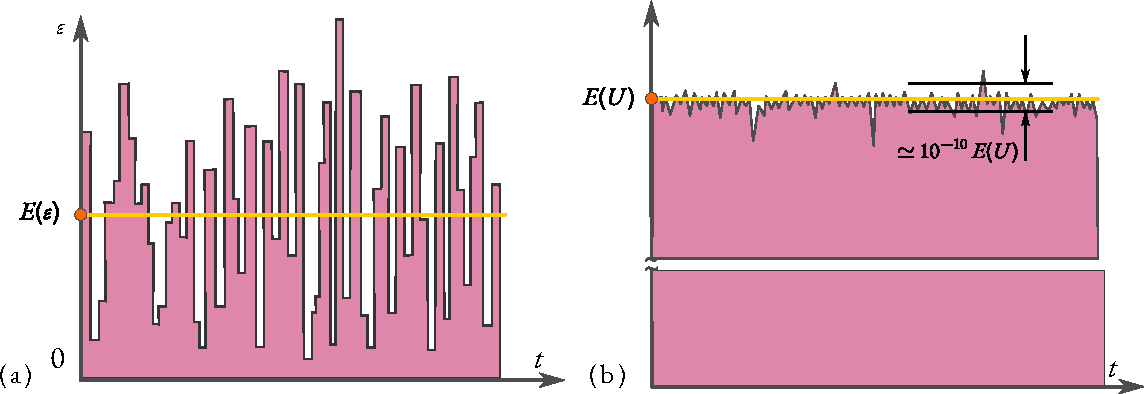
\includegraphics[width=1.4\textwidth]{figures/macro-micro.pdf}
\sidecaption{A comparison of the fluctuations of the micro-variable	$\varepsilon$ and	macro-variable $U$.\label{macro-micro}}
% fig 4.11
\end{figure*}

Thus, the total internal energy $U$ is not a fixed value for an equilibrium state of a macroscopic body. It varies slightly in time, going through small fluctuations around its mean value. Temperature, pressure, and entropy fluctuate around their mean values too.


\txthead{Brownian movement.} Having seen \eqref{eq-4.43}, a reader may conclude that under ordinary conditions, i.e. when we deal with macroscopic bodies and the macro-variables characterizing them, fluctuations do not show themselves. However, we can actually observe fluctuations by eye. Consider the \redem{Brownian movement} as an example.

In 1827, the English biologist Robert Brown (1773-1858) used a microscope to study small particles (plant pollen) suspended in water. He discovered that they were in constant chaotic motion. He was sure that this movement was due to the particles themselves rather than a result of flows in the liquid or its evaporation.

A correct explanation of Brownian movement was given in 1905 by Albert Einstein (1879-1955). He showed that the cause of the Brownian movement is the chaotic bombardment of the small suspended particles by the molecules of the surrounding liquid.

Imagine a small disc with a diameter of, for instance, \SI{d-4}{\centi\meter} suspended in a liquid. The number of collisions between the liquid molecules and one side of the disc per unit time equals, on average, the number of collisions on the other side. But this is only on the average. In reality, the number of collisions on one side of the disc during a small interval of time may be noticeably greater than the number of collisions on the other side. The result is that the disc receives an overall unbalanced impulse and so moves in the appropriate direction. We can say that the disc moves because of the \redem{fluctuations in the pressure} exerted by the liquid molecules on the two sides of the disc.

Einstein considered a concrete physical model with a ball as a Brownian particle. He showed that the mean square of the displacement of such a particle during an observational period $\tau$ is defined by the following formula
\begin{equation}%
E(l^{2}) = \frac{\tau}{8 \pi \eta r} k T,
\label{eq-4.44}
\end{equation}
where $r$ is the ball's radius, $\eta$ is the viscosity coefficient of the liquid, $T$ is its temperature.

\txthead{Why the sky is blue.} The colour of the sky is due to the diffusion of sunlight through the Earth's atmosphere. Let us imagine the atmosphere to be separated into a great number of small cubic cells each with an edge a wavelength of light long (about \SI{0.5d-4}{\centi\meter}), The chaotic motion of the air molecules results in that the number of molecules within the cell varies randomly from cell to cell. It will also vary randomly within a cell if we observe it at different instants in time. Sunlight diffuses through these \redem{fluctuations of air density}.

The intensity $\Delta I$ of light diffused through a volume of air $\Delta V$ at distance $R$ from the observer is defined by the relationship
\begin{equation}%
\Delta I = a \frac{\Delta V}{R^{2}} \frac{1}{\lambda^{4}} kT,
\label{eq-4.45}
%eq 4.45
\end{equation}
where $\lambda$ is the light wavelength, $T$ is the air temperature, and $a$ is a factor we shall not deal with here. It is clear from \eqref{eq-4.45} that the shorter the wavelength the more light diffuses ($\Delta I \propto \lambda^{4}
$). Therefore, the spectrum of the light which diffuses through the Earth's atmosphere proves to have a peak at the \redem{shortwave end}, which explains why the sky is \bluq{blue}.

\txthead{The Nyquist formula.} It follows from Ohm's law that if there is no electromotive force in an electric circuit, there is no current in it. However, this is not quite true. The point is that fluctuations related to the thermal movement of electrons in a conductor result in fluctuating currents, and hence a fluctuating electromotive force. In 1927, the American physicist and engineer Harry Nyquist (1889-1976) showed that if there is a conductor with resistance $R$ and temperature $T$, a \redem{voltage fluctuation} $\delta V$ appears at the ends of the resistor, the mean square of the fluctuation being
\begin{equation}%
E(\delta V)^{2} = 4 R k T \Delta \nu,
\label{eq-4.46}
\end{equation}
where $\Delta \nu $ is the range of frequencies within which the voltage fluctuations are measured.

Fluctuating electrical variables play an essential role in modern technology. They are, in principle, an unavoidable source of noise in communication channels and define the sensitivity limits of measuring instruments. Besides fluctuations caused by the thermal motion of electrons in conductors, let me mention another essential type of fluctuation, the fluctuation in a number of electrons leaving the heated cathode of an electron tube.

\txthead{Fluctuations and temperature.} I would like to draw the reader's
attention to expressions \eqref{eq-4.35} and \eqref{eq-4.35}. It is clear that a quadratic fluctuation is related to the absolute temperature: $\sqrt{\text{var}} \propto T$. The same result can be derived from formulas \eqref{eq-4.44}-\eqref{eq-4.46}. The relation between the quadratic fluctuation of a physical variable and temperature has a deep meaning. The greater the temperature of a body the more a physical parameter will fluctuate.

We noted above that the temperature of a body can be regarded as a measure of the average energy of the body's particles. Recall that this is only valid if the body is in thermal equilibrium. If an ensemble of particles is very far from equilibrium (suppose we are discussing a cosmic shower or the beam of particles from an accelerator), then the average energy of the particles cannot be measured by temperature. A more general approach to the notion of a body's temperature is its relation with the fluctuations of its physical parameters rather than the average energy of its particles. Temperature can be regarded as a measure of fluctuation. By measuring the fluctuations, we can measure the absolute temperature of the body in principle. The fluctuations in the electrical variables suit this purpose best.

The relationship between temperature and fluctuations indicates, in particular, that the notion of temperature, strictly speaking, has no analogue in Newtonian mechanics. Temperature involves probabilistic processes and is a measure of the variance of random variables.

\section{Entropy and Probability }

\txthead{From the formula of the work done by a gas during an isothermal expansion to Boltzmann's formula.} Suppose an ideal gas with mass $m$ and temperature $T$ expands isothermally from volume $V_{1}$ to volume $V_{2}$. According to \eqref{eq-4.6}, the work performed by the gas during the expansion is $(mRT/ M) \, \ln \,(V_{2}/ V_{1})$. During an isothermal expansion, the work is done due to a quantity of heat $Q$ drawn by the gas from the environment. Therefore,
\begin{equation}%
Q =	\frac{mRT}{M} \, \ln \, \left( \frac{V_{2}}{V_{1}} \right).
\label{eq-4.47}
\end{equation}
Using \eqref{eq-4.24} for the equation of state of an ideal gas, we can transform \eqref{eq-4.47} into
\begin{equation}%
Q =	N k T \, \ln \, \left( \frac{V_{2}}{V_{1}} \right),
\label{eq-4.48}
\end{equation}
where $N$ is the number of molecules in the gas. Taking into account \eqref{eq-4.10}, we can conclude that the increment of entropy in the gas is
\begin{equation}%
\Delta S =	N k \, \ln \, \left( \frac{V_{2}}{V_{1}} \right).
\label{eq-4.49}
\end{equation}
The isothermal expansion of a gas is a \redem{reversible} process. The increase of entropy in a reversible process should not surprise the reader: we consider the entropy of a gas, and the gas here is an open system (it performs work on a piston or draws heat from an external body). The same increase in entropy is observed in an \redem{irreversible} process of gas expansion from $V_{2}$ to $V_{1}$ when the gas is a closed system. This irreversible process can be carried out as follows. Suppose that a thermally insulated vessel of volume $V_{0}$ has a partition, and first all the gas is on one side of the partition and occupies volume $V_{1}$. Then the partition is removed and the gas expands into vacuum. The expansion is considered to start when the partition is removed and to end when the gas occupies volume $V_{2}$. The increment in the gas's entropy during this process is also defined by formula \eqref{eq-4.49}.

Using the example of gas expansion into a vacuum, we can explain the increase in entropy on the basis of \redem{probabilities}. The probability that a gas molecule occurs in volume $V_{1}$ is evidently equal to $V_{1} / V_{0}$. The probability that another molecule will occur in volume $V_{1}$ simultaneously with the first one is $(V_{1} / V_{0})^{2}$. The probability that all $N$ molecules
will gather in volume $V_{1}$ is $(V_{1} / V_{0})^{N}$. Let us use $w_{1}$ to denote the probability that all molecules are in volume $V_{1}$ and $w_{2}$ to denote the probability that all molecules will occur in volume $V_{2}$. The first probability is $(V_{1} / V_{0})^{N}$ while the second one is $(V_{2} / V_{0})^{N}$. Therefore,
\begin{equation}%
\frac{w_{2}}{w_{1}} =	 \left( \frac{V_{2}}{V_{1}} \right)^{N}.
\label{eq-4.50}
\end{equation}
We can therefore obtain from \eqref{eq-4.49}:
\begin{equation}%
\Delta S =	N k \, \ln \, \left( \frac{V_{2}}{V_{1}} \right) = k \, \ln \, \left( \frac{V_{2}}{V_{1}} \right)^{N} = k \, \ln \, \left( \frac{w_{2}}{w_{1}} \right).
\label{eq-4.51}
\end{equation}
Thus, using rather simple reasoning, we have arrived at an essential result, namely Boltzmann's formula.

\txthead{Boltzmann's formula.} In 1872, Ludwig Boltzmann (1844-1906) published a formula in which the entropy of a system in a certain state is proportional to the \redem{logarithm of the probability of the state}. The proportionality factor in this formula was refined later and was called \redem{Boltzmann's constant}. Boltzmann's equation is now given as
\begin{equation}%
S= k \, \ln \, w.
\label{eq-4.52}
\end{equation}
Formula \eqref{eq-4.51} is obtained from \eqref{eq-4.52} if we assume that $S_{1}= k \, \ln \, w_{1}$, $S_{2}= k \, \ln \, w_{2}$, and $\Delta S = S_{2} - S_{1}$.

Suppose a system consists of two subsystems, one of which is in state
$\mathit{1}$ with entropy $S_{1}$ and probability $w_{1}$ and the other is in state $\mathit{2}$ with entropy $S_{2}$ and probability $w_{2}$.	Let	$S$ and $w$ be the entropy and	the probability of the entire system's state, respectively. Entropy is additive, and therefore
\begin{equation}%
 S= S_{1} + S_{2}.
\label{eq-4.53a}
\tag{4.53a}
\end{equation}
This state is realized when the first subsystem is in state $\mathit{1}$ and the second subsystem is in state $\mathit{2}$ at the same time. According to the theorem of probability multiplication,
\begin{equation}%
w = w_{1} \cdot w_{2}.
\label{eq-4.53b}
\tag{4.53b}
\end{equation}
It is clear that \eqref{eq-4.53a} and \eqref{eq-4.53b}) are in agreement with Boltzmann's formula:
\begin{equation*}%
S= k \ln ( w_{1} \, w_{2}) = k \ln  w_{1}  +k \ln \, w_{2} = S_{1} + S_{2}.
\end{equation*}

\txthead{Macro-states and micro-states.} Now what is the ``probability of the system's state''? Consider a simple system consisting of four particles, each of which may be in either of two states with equal probability. We can imagine a vessel divided into two equal parts (left and right) and only four molecules inside the vessel. Each of the molecules may be found in the left or right half with equal probability. This system has five possible macro-states: $\mathit{1}$, there are no molecules in the left half; $\mathit{2}$, there is one molecule in the left half; $\mathit{3}$, there are two molecules in the left half; $\mathit{4}$, there are three molecules in the left half; and $\mathit{5}$, there are four molecules in the left half. These macro-states may be realized by \redem{different numbers of equally probable ways}, or, in other words, different macro states correspond to different numbers of micro-states. This is clear from \figr{entropy-disorder}, where different colours are used to mark the different molecules. We can see that macro-states $\mathit{1}$ and $\mathit{5}$ may only occur in one way each. Each therefore corresponds to one micro-state. Macro-states $\mathit{2}$ and $\mathit{4}$ correspond to four micro-states. Macro-state $\mathit{3}$ corresponds to six equally probable micro-states. There can be 16 equally probable micro-states in all. The probability of a macro-state is \redem{proportional to the number of corresponding micro-states}, and this is the probability involved in Boltzmann's formula. The number of micro-states corresponding to a given macro-state is called its \redem{statistical weight}.

\begin{figure}[!ht]
 \centering
 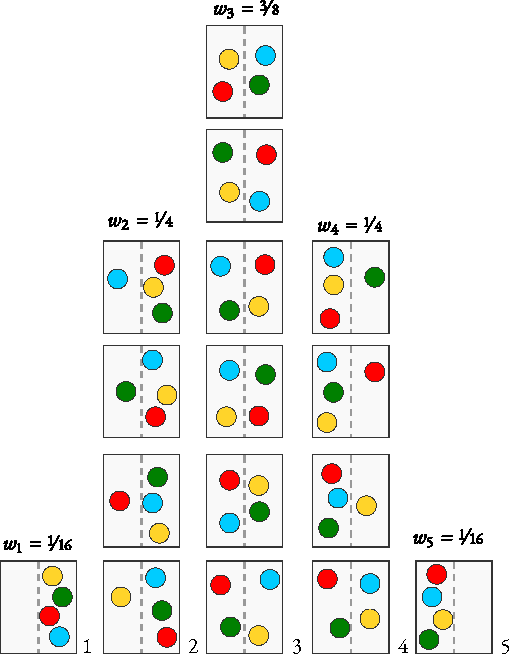
\includegraphics[width=0.7\linewidth]{figures/macro-state-1.pdf}
\sidecaption{Entropy as a measure of disorder in the system.\label{entropy-disorder}}
%fig-12
 \end{figure}
 
Suppose that there are $N$ molecules rather than four in the vessel divided into two equal halves. Now there are $N + 1$ macro-states, which can	 be	conveniently designated	by	the	numbers	$0, 1,2, 3, \ldots , N$, according to the number of molecules present, say, in the left half. The statistical weight of the $n^{\text{th}}$ macro-state equals the number of combinations of $N$ things taken $n$ at a time:
\stepcounter{equation}
\begin{equation}%
\begin{pmatrix}
N\\ n
\end{pmatrix}= \frac{N!}{(N-n)! \,n!}.
\label{eq-4.54}
\end{equation}
This is the number of micro-states corresponding to the $n^{\text{th}}$ macro-state.

The total number of micro-states is defined by the sum 
\begin{equation*}
\sum_{n=0}^{N} \begin{pmatrix}
N\\ n
\end{pmatrix}
\end{equation*}
The probability of the $n^{\text{th}}$ macro-state is
\begin{equation}%
w_{n} = \left. \begin{pmatrix}
N\\ n
\end{pmatrix} \middle/ \sum_{n=0}^{N} \begin{pmatrix}
N\\ n
\end{pmatrix} \right.
\label{eq-4.55}
\end{equation}

\txthead{An example using Boltzmann's formula.} Suppose a gas consisting of $N$ molecules expands into vacuum. Its volume doubles. Find the increase in the gas's entropy.

The \redem{initial} state of the gas is the macro state with $n = 0$ (all molecules are in the right half of the vessel), and the final state is the macro-state with $n = N /2$ (the molecules are uniformly distributed	between both halves of the vessel, which means the volume of the gas has doubled). Here we assume that $N$ is an even number (this reservation is not essential for large $N$). In agreement with \eqref{eq-4.54} and \eqref{eq-4.55}, we can write:
\begin{equation}%
\frac{w_{N/2}}{w_{0}} = \left. \begin{pmatrix}
N\\ N/2
\end{pmatrix} \middle/  \begin{pmatrix}
N\\ 0
\end{pmatrix} \right.
= \begin{pmatrix}
N\\ N/2
\end{pmatrix} = \frac{N!}{(N/2)! \, (N/2)!}.
\label{eq-4.56}
\end{equation}
According to Boltzmann's formula, the increase in the gas's entropy is
\begin{equation}%
\Delta S = k \, \ln \,\frac{w_{N/2}}{w_{0}} = k \ln \, \frac{N!}{(N/2)! \, (N/2)!},
\label{eq-4.57}
\end{equation}
Since $N$ is a very large number, we can use the approximation
\begin{equation}%
\ln (N!) = N \ln N,
\label{eq-4.58}
\end{equation}
hence \eqref{eq-4.57} takes the form 
\begin{equation}%
\Delta S = k N \ln 2.
\label{entropy-4}
% eq 4.59
\end{equation}
The same result follows from \eqref{eq-4.49} if we assume $V_{2} / V_{1} = 2$. 

\txthead{Entropy as a measure of disorder in a system.} Let us return to \figr{entropy-disorder}. Macro-states $\mathit{1}$ and $\mathit{5}$ clearly show the structure of the system, its separation into two halves. There are molecules in one half and no molecules in the other. On the contrary, macro-state $\mathit{3}$ does not have this structure at all because the molecules are evenly distributed in both halves. The presence of a definite structure is related to the \redem{order} in a system while the absence of structure is related to \redem{disorder}. The greater the degree of order in a macro-state, the smaller its statistical weight (i.e. the number of corresponding micro-states is smaller). Disordered macro-states with no inner structure have large statistical weight. They can be realized in many ways, in other words, by many micro-states.

All this allows us to regard entropy as a \redem{measure of disorder in a system}. If the disorder in a given macro-state is large, its statistical weight is large, and therefore, its entropy is large.



\txthead{A statistical explanation of the second law of thermodynamics.} Boltzmann's formula makes it possible to explain the increase in entropy during irreversible processes in a closed system as postulated by the second law of thermodynamics. The \redem{increase in entropy} means the transition of the system from a \redem{less probable} state to a \redem{more probable} one. The example of gas expanding into vacuum illustrates this. While the gas expands, the system moves from a less probable to a more probable macro-state.

Any process in a closed system proceeds in a direction such that the system's entropy does not decrease. This means that transitions to more probable states or, at least, transitions between equally probable states correspond to real processes.

When a probabilistic approach is used entropy becomes a measure of the disorder in a system. The law requiring the increase of the entropy in a closed system is, therefore, a law which demands that the \redem{degree of disorder} in these systems increases. In other words, a transition from a less probable to a more probable state corresponds to an order-disorder transition. For instance, when a hammer strikes an anvil, the ordered component of the hammer's molecular movement related to its overall downward movement is transformed into the disordered thermal molecular movement of the anvil and the hammer.

The \redem{quantity} of energy in a closed system does not vary in time. However, the \redem{quality} of the energy varies. In particular, its capacity to perform usable work decreases. The increase of entropy in a closed system is, in its essence, a gradual destruction of the system. Any closed system is unavoidably disordered and degraded as time passes. The isolation of a system subjects it to the power of destructive chance, which always sends the system into disorder. As the French scientist Leon Brillouin once said, ``the second law of thermodynamics means death due to isolation''. 

Maintaining or, moreover, increasing the order in a system requires
that the system be \redem{controlled}, for which it is necessary, first of all, that the system should \redem{not be isolated} or closed. Naturally, when the system loses its ``protecting envelope'', it is open to external disorganizing factors. However, it also becomes available to control factors. The action of the latter can decrease the system's entropy. Of course, this does not contradict the second law of thermodynamics: the decrease of entropy is local in nature, only the entropy of the given system decreases. This decrease is more than compensated by an increase in the entropy in other systems, in particular, those that control the given system.

\txthead{Fluctuations and the second law of thermodynamics.} The probabilistic approach both explained the second law of thermodynamics and showed that the demands of this law are not absolute. The direction in which II process must proceed is dictated by the second law, but it is not strictly predetermined. It is only the \redem{most probable} direction. In principle, violations of the second law of thermodynamics are possible. However, we do not observe them because their \redem{probability is low}.

A gas expands into vacuum spontaneously. This is the most probable direction of the process. However, there is another possible situation, viz. the velocities of the molecules in the gas suddenly point in directions such that the gas spontaneously compresses. This situation has an exceptionally low probability because of the enormous number of molecules in any macro-volume of gas. The spontaneous compression of the gas should be regarded as a fluctuation of its density. If the number of molecules in the gas is large, then, as is known, the characteristic value of the relative fluctuation is small (recall that it is proportional to $1 / \sqrt{N}$), and therefore, it is very improbable that a fluctuation on the scale of the macrocosm would be observed.

Suppose a phenomenon requires the participation of a relatively small number of molecules. Then it is not difficult to observe various kinds of fluctuations that violate the second law of thermodynamics. In the preceding section, we discussed density fluctuations in air inside volumes
whose linear dimensions are comparable to the light wavelengths. These fluctuations appear as spontaneous compressions and rarefactions in the air, bringing about the blue colour of the sky.

It is most probable for a Brownian particle to collide with the same number of liquid molecules on both sides per unit time. However, because of the small dimensions of the Brownian particle, fluctuations of pressure due to unbalanced number of collisions from different directions are quite probable such that the particle will randomly move. A moving Brownian	particle demonstrates the	spontaneous transformation of heat taken from a liquid into the kinetic energy of the particle's motion.

Therefore, we see that the probabilistic explanations of entropy and the second law of thermodynamics help comprehend more deeply the nature of processes in macro-systems. The probabilistic approach explains the puzzles thermodynamics could not solve and, moreover, indicates that the second law of thermodynamics itself has the \redem{probabilistic nature} because it is only valid on the average, and various fluctuations violate this law of thermodynamics. We come to an essential conclusion: 
\begin{mybox}{}
probabilistic laws rather than strictly deterministic ones underlie the second law of thermodynamics.
\end{mybox}



\section{Entropy and Information }

\txthead{The relation between entropy and information.} It was shown in Chapter 3 that the notion of information is underlain by probability. Now we have seen that probability is the basis of entropy. The unity of the nature of \redem{information} and \redem{entropy} proves to be essential. An increase in the entropy of a system corresponds to its transition from a less ordered state to a more ordered one. This transition is accompanied by a decrease in the information contained in the structure of the system. Disorder and uncertainty can be regarded as a lack of information. In turn, information is nothing else but a decrease in uncertainty.


According to the second law of thermodynamics, the entropy of a closed system increases in time. This process corresponds to the loss of information due to random factors, as was considered in Chapter 3. Fluctuations in physical parameters cause random violations of the second law of thermodynamics. Random decreases of entropy are observed. These processes correspond to the generation of information from noise which we discussed above. By influencing the system in a certain way, we can decrease its entropy (by increasing the entropy of another system). This is the process of control, which demands definite information.
All this speaks in favour of relation between information and entropy. The Hungarian physicist Leo Szilard (1898-1964) was first to indicate this relation, doing so in 1929.

Thus, \redem{entropy is a measure of disorder} and uncertainty in a system, and \redem{information is a measure of order} and structural certainty. An increase in information corresponds to a decrease in entropy and, vice versa, a decrease in information corresponds to an increase in entropy.

\txthead{Boltzmann's formula and Hartley's formula.} We came across Hartley's formula in Chapter~3 (see \eqref{eq-3.1}. According to this formula, the information required to indicate which of $N_{1}$ equally probable outcomes is wanted is $I= \log_{2} \, N_{1}$. Suppose $N_{1}$ is the number of railroad tracks at a station. The signalman has to send a signal indicating the track along which the train is to approach the station. Sending the signal, the signalman selects from $N_{1}$ equally probable outcomes. This signal contains  $I_{1} = \log_{2} \, N_{1}$ bits of	information. Now suppose	that	some of the tracks must be repaired, so that the signalman must select from $ N_{2}$ outcomes ($ N_{2} <  N_{1}$). Now his signal contains information $I_{2} = \log_{2} \, N_{2}$ The difference
\begin{equation}%
\Delta I = I_{1}- I_{2} = \log_{2} \, \left( \frac{N_{1}}{N_{2}} \right),
\label{eq-4.60}
\end{equation}
is information about the repair of the tracks. In other words, this is the information required to decrease the number of equally probable outcome	from $N_{1}$ to $ N_{2}$.

Let us compare the existence of $N$ equally probable outcomes with the presence of $N$ equally probable micro-states, i.e. with the statistical weight $N$ of a certain macro-state. According to Boltzmann's formula, a decrease in the statistical weight of a macro-state from $N_{1}$ to $ N_{2}$ means that the system's entropy is incremented by
\begin{equation}%
\Delta S = - k  \ln \, \left( \frac{N_{1}}{N_{2}} \right).
\label{eq-4.61}
\end{equation}
I used a minus sign here because the entropy decreases (the increment is negative) as the statistical weight decreases. In compliance with \eqref{eq-4.60}, to realize this negative entropy requires an increment in the information of $\Delta N = I_{1}- I_{2} = \log_{2} \, \left( N_{1}/ N_{2} \right)
$.Comparing \eqref{eq-4.60} with \eqref{eq-4.61} and given that
\begin{equation*}
\log_{2} \, \left( \frac{N_{1}}{N_{2}} \right) = \frac{\ln \left( N_{1}/ N_{2} \right) }{\ln \, 2}.
\end{equation*}
Therefore, an increment in the information $\Delta \, I$ corresponds to a decrease in the system's entropy of $\Delta \, I \, k / \ln \, 2$.

Norbert Wiener called information to be negative entropy. Louis Brillouin suggested using the term ``negentropy'' rather than ``negative entropy''.

\txthead{Maxwell's demon and its exorcism.} In 1871, Maxwell formulated the following paradox. Suppose a vessel with a gas is separated into two halves ($A$ and $B$) by a partition with a trapdoor over a microscopic hole in it. And suppose, Maxwell continued, a ``being'' (Maxwell called it a ``demon'') controls the trapdoor causing it to close and open the hole so as to let the fastest molecules from the $A$ half of the vessel enter the $B$ half and to let the slowest molecules from the $B$ half into the $A$ half. Thus, the demon would increase the temperature in the $B$ half and decrease it in the $A$ half without doing any work, which evidently contradicts the second law of thermodynamics.
\begin{figure}[!ht]
 \centering
 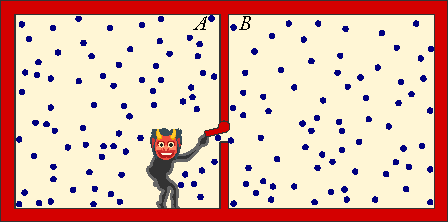
\includegraphics[width=0.9\linewidth]{figures/maxwell-demon.pdf}
\sidecaption{Maxwell's demon controls the flow of molecules from one section to another.\label{max-demon}}
 \end{figure}
When looking at the illustration of Maxwell's demon (\figr{max-demon}), the reader clearly should not think of an evil force. The point of contention is a device that opens and closes a hole in the way the demon described above would act.

Three types of device could be suggested in principle. The first type would be a device controlled by the gas molecules present in the vessel. Imagine there is a one-way trapdoor which responds to the energy of the molecules striking it: fast molecules open the door and slow ones do not. So that it open when struck by an individual molecule, the door would have to be exceedingly light. However, such a door, if it could be produced, would be unable to carry out the functions of the demon. The door would in fact be affected both by the fluctuations due to the motion of the gas molecules and by the fluctuations related to the thermal motion of the molecules of the material making up the door. The door would therefore operate chaotically and would not sort molecules by speed.

The second type of demon would be a device controlled from the outside. Suppose we could monitor the molecules arriving at the hole in the partition. The monitoring device would signal at the right moment and the trapdoor would open or close. If we ignore the technical problems, we might have to admit that this way of sorting the molecules is possible in principle. However, it will not be a substitute for Maxwell's demon because the latter should work in a \redem{closed} system.

This is essential because it is a decrease in the entropy of a closed system that violates the second law of thermodynamics. But our system is open, the ``demon'' obtaining information from the outside. The reception of information must be regarded as an inflow of negative entropy (negentropy) into the system, which is equivalent to a decrease in the system's entropy.

There is one more type of the demon, an \redem{intelligent} demon. However, such a demon would not be what we are looking for because, as Einstein said, an intelligent mechanism cannot act in an equilibrium medium. In other words, life and intelligence are impossible in a closed system, that is in a state of equilibrium.

\txthead{Entropy and life.} A living organism is a very ordered system with low entropy. The existence of living organisms suggests a continuous maintenance of the system's entropy at a low level, a continuous reaction to disordering factors, and, in particular, the factors causing diseases. It may seem that an organism does not obey the demands of the second law of thermodynamics.

Naturally, this is not so. We should take into account that any organism is an \redem{open} system in an essentially \redem{non-equilibrium} state. This system actively interacts with its environment, continuously drawing negentropy from it. For instance, it is well-known that food has lower entropy than waste.

Man does not just live. He works, creates, and therefore, actively decreases entropy. All this is only possible because man obtains negentropy (information) from the environment. It is supplied to him via two different channels. The first one is related to the process of learning. The second channel is related to physiological processes of metabolism occurring in the ``man-environment'' system.


%%% Local Variables:
%%% mode: latex
%%% TeX-engine: xetex
%%% TeX-master: "twibop2"
%%% End:
